% \documentclass[a4paper,10pt]{article}
\documentclass[review]{siamart}
\usepackage{url}
\usepackage{amssymb}
\usepackage{amsmath}
\usepackage{bm}
\usepackage{stmaryrd}
\usepackage{array}
\usepackage{empheq}
\usepackage{enumitem}
	\setlist{nosep} % or \setlist{noitemsep} to leave space around whole list
\usepackage{color}
%\usepackage{showlabels}
\usepackage{adjustbox}
\usepackage{hyperref}
\hypersetup{
  colorlinks   = true, %Colours links instead of ugly boxes
  urlcolor     = blue, %Colour for external hyperlinks
  linkcolor    = blue, %Colour of internal links
  citecolor   = red %Colour of citations
}
\usepackage[numbers,sort]{natbib}
\usepackage{cleveref}

\newsiamremark{remark}{Remark}


% \newtheorem{lemma}{Lemma}
% \newtheorem{definition}{Definition}
% \newtheorem{theorem}{Theorem}
% \newtheorem{corollary}{Corollary}

\newcommand{\tcb}{\textcolor{blue}}
\newcommand{\tcp}{\textcolor{purple}}
\newcommand{\todo}[1]{\textcolor{red}{[TODO\@: #1]}}

\newcommand{\mdet}{\operatorname{det}}
\newcommand{\madj}{\operatorname{adj}}

% ------------------------------------------------------------------------------------ %
% ------------------------------------------------------------------------------------ %

\newcommand{\TheTitle}{IRK!}
\newcommand{\TheAuthors}{B.S. Southworth }
\headers{IRK!}{\TheAuthors}
\title{{\TheTitle}\thanks{This research was conducted ...
  }}

\author{%
  Ben~S.~Southworth
  \thanks{Department of Applied Mathematics,
          University of Colorado at Boulder
          (\email{ben.s.southworth@gmail.com}).}
}

\ifpdf%
\hypersetup{%
  pdftitle={\TheTitle},
  pdfauthor={\TheAuthors}
}
\fi

% ------------------------------------------------------------------------------------ %
% ------------------------------------------------------------------------------------ %

\begin{document}
\allowdisplaybreaks


% ------------------------------------------------------------------------------------ %
% ------------------------------------------------------------------------------------ %
% ------------------------------------------------------------------------------------ 
\newpage
\newpage
\section{Nonlinear}
Have ODEs,
%
\begin{align}
	M\mathbf{u}'(t) =  \mathcal{N}(\mathbf{u},t) \quad\text{in }(0,T], \quad \mathbf{u}(0) = \mathbf{u}_0,
\end{align}
%
where $M$ is a mass matrix and $\mathcal{N} \colon \mathbb{R}^{N} \times \mathbb{R}_+ \to \mathbb{R}^{N}$ is a discrete, time-dependent, nonlinear operator. Then, an $s$-stage IRK scheme approximately propagates the discrete  solution by
%
\begin{align}
\mathbf{u}_{n+1} & = \mathbf{u}_n + \delta t \sum_{i=1}^s b_i\mathbf{k}_i,
\end{align}
with stage vectors satisfying the block system of $s$ nonlinear equations,
\begin{align}
M\mathbf{k}_i & = \mathcal{N}\left(\mathbf{u}_n + \delta t\sum_{j=1}^s a_{ij}\mathbf{k}_j, t_n+\delta tc_i\right), \quad i = (1,\ldots,s).
\end{align}

For a given pair $(\bm{u}_n,t_n)$, let's define the operator $F_i \colon \mathbb{R}^{sN} \to \mathbb{R}^N$ that encodes the $i$th stage vector,
\begin{align}
F_i(\bm{k}) \coloneqq M \bm{k}_i - {\cal N} \left(\bm{u}_n + \delta t \sum \limits_{j = 1}^s a_{ij} \bm{k}_j, t_n + c_i  \delta t \right),
\end{align}
with $\bm{k} = (\bm{k}_1, \ldots, \bm{k}_s)^\top$ the vector of stages. Then, the nonlinear system we need to solve to advance forwards one time step is
\begin{align}
\begin{bmatrix}
F_{1}(\bm{k})\\
\vdots \\
F_{s}(\bm{k})
\end{bmatrix}
\eqqcolon F(\bm{k}) = 0.
\end{align}
%
%Let's say we solve this system via a Newton-type method. That is, we apply a fixed-point algorithm like 
%\begin{itemize}
%\item Given initial iterate $\bm{\hat{k}} \approx \bm{k}$, if $\Vert F(\bm{\hat{k}}) \Vert > \varepsilon$, 
%\item Solve $G(\bm{\hat{k}}) \bm{d} = - F(\bm{\hat{k}})$, where $G(\bm{x}) \approx F'(\bm{x})$ is some approximation of the Jacobian of $F$ evaluated at $\bm{x}$
%\item Update iterate $\bm{\hat{k}} \to \bm{\hat{k}} + \bm{d}$ 
%\item If $\Vert F(\bm{\hat{k}}) \Vert > \varepsilon$, repeat
%\end{itemize}
%
%The particular method will be defined by the approximate Jacobian, $G$. Note the true Jacobian matrix is
%\begin{align}
%F'(\bm{\hat{k}}) = 
%\begin{bmatrix} M \\ 
%& \ddots \\ 
%& & M
%\end{bmatrix}
%- 
%\delta t
%\begin{bmatrix} {\cal L}_1 \\ 
%& \ddots \\ 
%& & {\cal L}_s
%\end{bmatrix}
%(A_0 \otimes I)
%\end{align}
%where
%\begin{align}
%{\cal L}_i \coloneqq {\cal N}' \left(\bm{u}_n + \delta t \sum \limits_{j=1}^s a_{ij} \bm{\hat{k}}_j, t_n + c_i \delta t \right).
%\end{align}
%
%In the formulation, we factor out a part of the Schur decomposition of $A_0 = Q_0 R_0 Q_0^\top$, and, so the linear systems we actually solve during a Newton-like step take the form
%\begin{align}
%\big[ R_0 \otimes M - (Q_0^\top \otimes  I) L (Q_0 \otimes I) \big] 
%(R_0^{-1} Q_0^\top \otimes I) \bm{d} = - (Q_0^\top \otimes I) F( \bm{k}^0).
%\end{align}
%where $L \approx {\rm diag}({\cal L}_1, \ldots, {\cal L}_s)$.
%
%During each Newton iteration, we first solve the system
%\begin{align}
%\big[ R_0 \otimes M - (Q_0^\top \otimes  I) L (Q_0 \otimes I) \big]  \bm{z} = \bm{y}
%\end{align}
%via backward substitution, where $ \bm{y} = - (Q_0^\top \otimes I) F( \bm{k}^0)$. Then we solve for $\bm{d} = (Q_0 R_0 \otimes I) \bm{z}$ via simple multiplication.



\tcp{But rather than solving this nonlinear system, we make a slight change of variables.}
Say we make the following simple change of variables:
\begin{align}
\bm{w} = (A_0 \otimes I) \bm{k} 
\quad 
\Longleftrightarrow 
\quad
\bm{k} = (A_0^{-1} \otimes I) \bm{w}
\end{align}
and we first solve the nonlinear problem for $\bm{w}$, then solve a linear problem to obtain $\bm{k}$ from $\bm{w}$ (well, we'd actually obtain $(\bm{b}_0^\top \otimes I) \bm{k} = (\bm{b}_0^\top A_0^{-1} \otimes I) \bm{w} = (\bm{d}_0^\top \otimes I) \bm{w}$ since this is what we really need). Now the nonlinear system becomes
\begin{align}
F(\bm{w}) = ( A_0^{-1} \otimes M ) \bm{w} - 
\begin{bmatrix}
{\cal N}(\bm{u}_{n} + \delta t \bm{w}_1, t_n + c_1 \delta t)\\
\vdots\\
{\cal N}(\bm{u}_{n} + \delta t \bm{w}_s, t_n + c_s \delta t)\\
\end{bmatrix}
= 
0.
\end{align}
What's interesting here is that the components of $\bm{w}$ are now only linearly coupled to each other (via the $A_0^{-1} \otimes M$ term), where with the previous formulation the components of $\bm{k}$ were nonlinearly coupled (every equation involves the evaluation the Jacobian of ${\cal N}$ with $(\bm{k}_i)_{i =1}^s$). The Jacobian is
\begin{align}
F'(\bm{w}) = A_0^{-1} \otimes M - 
\delta t
\begin{bmatrix} {\cal N}'_1 \\ 
& \ddots \\ 
& & {\cal N}'_s
\end{bmatrix}
\end{align}
where
\begin{align}
{\cal N}'_i \equiv {\cal N}' \left(\bm{u}_n + \delta t \bm{w}_i^0, t_n + c_i \delta t \right).
\end{align}

The linear systems we solve during the Newton-like solve take the form
\begin{align}
\big[ R_0 \otimes M - (Q_0^\top \otimes  I) (\delta t N')  (Q_0 \otimes I) \big] 
(Q_0^\top \otimes I) \bm{ \delta w } = - (Q_0^\top \otimes I) F( \bm{w}),
\end{align}
by using the Schur decomposition of $A^{-1}_0 = Q_0  R_0 Q^{\top}_0$ with block upper triangular $R_0$. And, 
\begin{align}
N' \approx  
\begin{bmatrix} {\cal N}'_1 \\ 
& \ddots \\ 
& & {\cal N}'_s
\end{bmatrix}.
\end{align}

\subsection{A simplified Newton}
We take
\begin{align}
N' = 
\begin{bmatrix} {\cal N}'_s \\ 
& \ddots \\ 
& & {\cal N}'_s
\end{bmatrix}
= 
I \otimes {\cal N}'_s,
\end{align}
such that the matrix 
\[\big[ R_0 \otimes M - (Q_0^\top \otimes  I) (\delta t N')  (Q_0 \otimes I) \big] = 
\big[ R_0 \otimes M - \delta t N' \big] \] is block upper triangular, and can be inverted via backward substitution. During this solve, we have to invert the diagonal blocks, which take the form (assuming  $M = I$)
\begin{align}
1 \times 1 \textrm{ systems:} \quad \zeta_j I - \delta t {\cal N}'_s,
\end{align}
and 
\begin{align}
2 \times 2 \textrm{ systems:} \quad
\begin{bmatrix}
\eta_jI  - \delta t {\cal N}'_s & \phi I \\
-\tfrac{\beta^2_j}{\phi}I & \eta_jI  - \delta t {\cal N}'_s \\
\end{bmatrix}
\end{align}

This is done with preconditioned GMRES, where for the $1 \times 1$ system, a single AMG iteration is applied to $\zeta_j I - \delta t {\cal N}'_s$. And for the 
$2 \times 2$ systems the preconditioner is 
\begin{align}
\begin{bmatrix}
\eta_jI  - \delta t {\cal N}'_s & 0 \\
-\tfrac{\beta^2_j}{\phi}I & \eta_jI  - \delta t {\cal N}'_s \\
\end{bmatrix}^{-1},
\end{align}
with the action of $(\eta_jI  - \delta t {\cal N}'_s)^{-1}$ approximated via a single AMG iteration.


We have some flexibility in terms of updating ${\cal N}'_s$. Some options:
\begin{enumerate}
\setlength\itemsep{0.5em}
\item Update at the start of every Newton solve (see Figure \ref{fig:simple_newton_convergence}, left panel)

\item Update every Newton iteration (See Figure \ref{fig:simple_newton_convergence}, right panel).
\end{enumerate}

\begin{figure}[H]
\centerline{
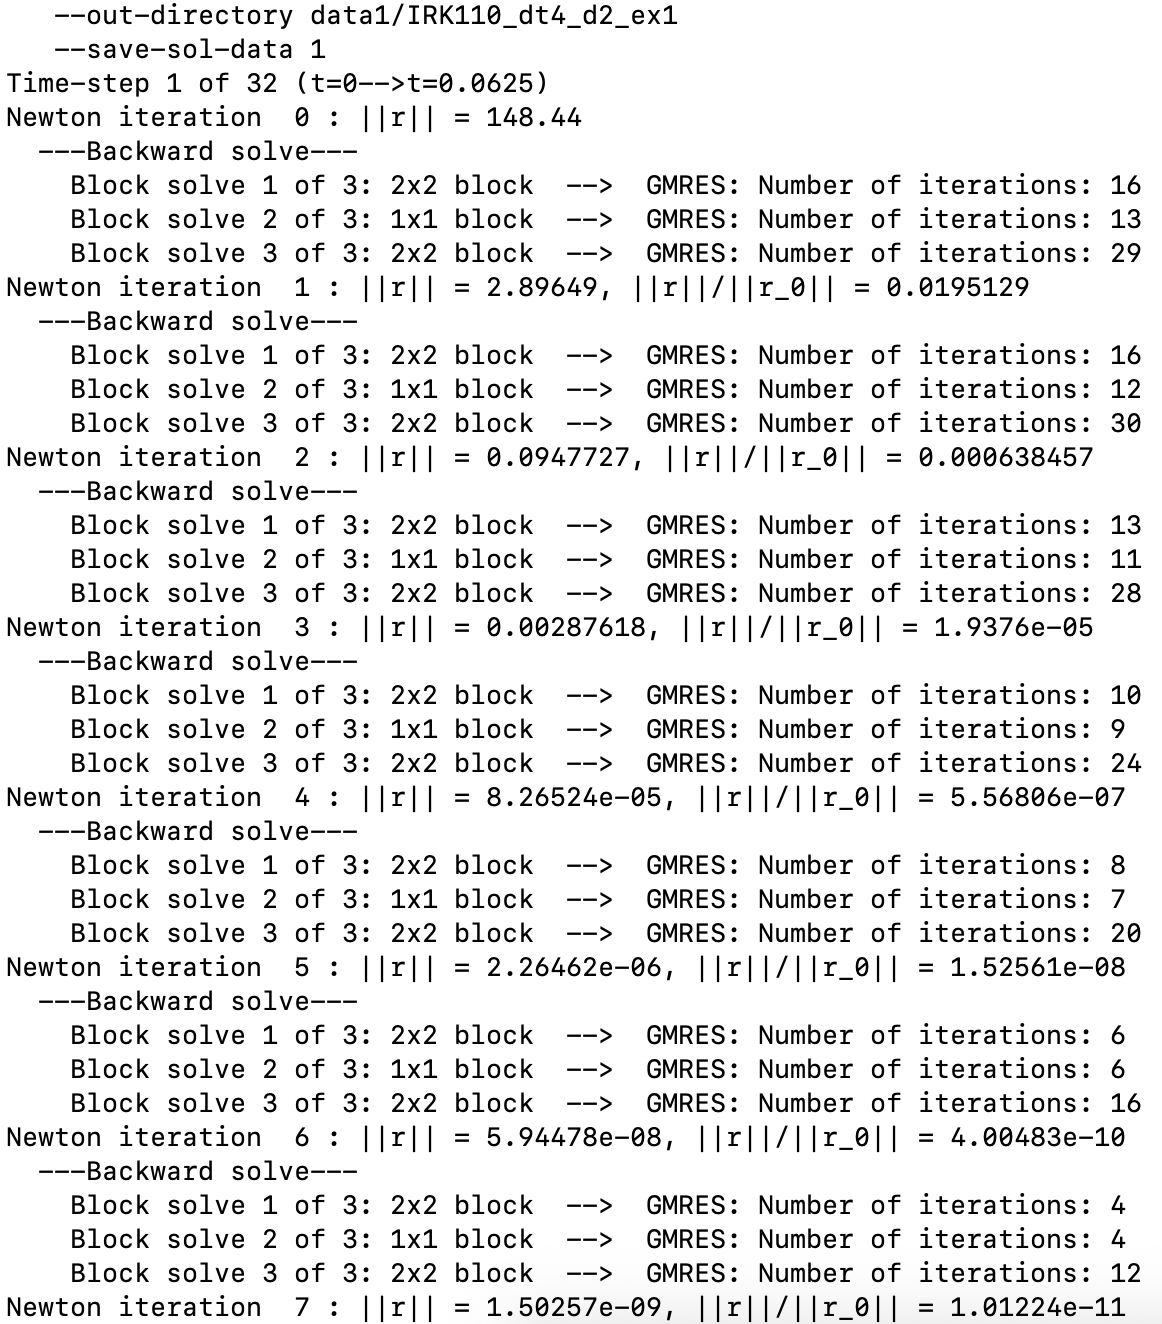
\includegraphics[width = 0.585\textwidth]{figures/simple_newton_basic}
\quad
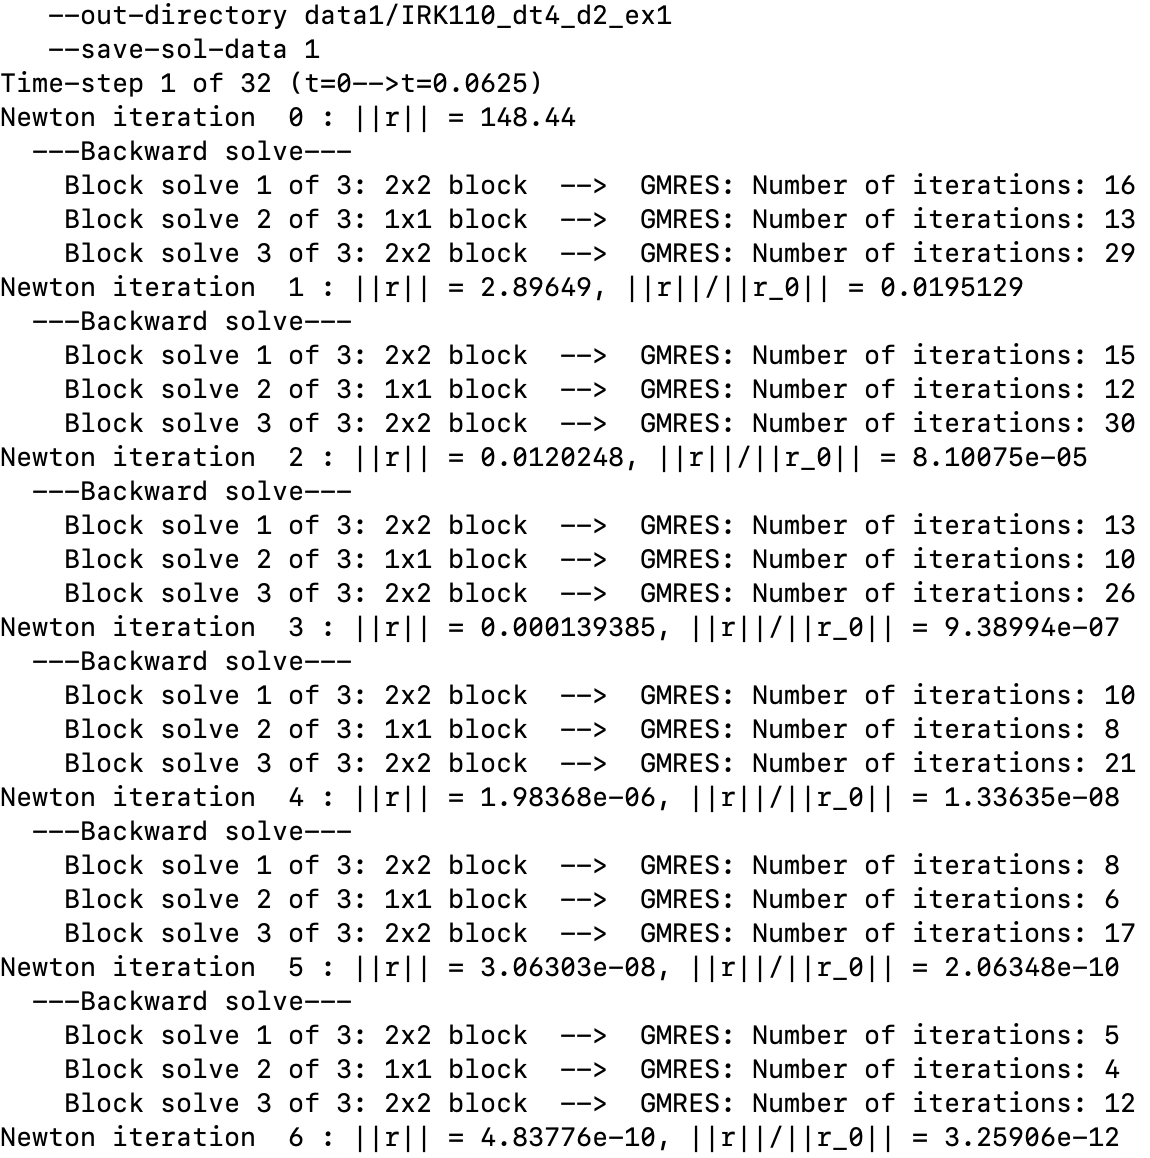
\includegraphics[width = 0.585\textwidth]{figures/simple_newton_better}
}
\caption{Simplified Newton convergence and that of its linear solver; first time step of finest resolution Gauss(10) solve from Figure \ref{fig:errors2D}.
\textbf{Left:} Jacobian fixed throughout Newton solve. \textbf{Right:} Updating approximate Jacobian each Newton iteration. Notice convergence on the \underline{right} is slightly faster.
\label{fig:simple_newton_convergence}
}
\end{figure}

\newpage
\section{Numerical results}

Numerically approximate the solution of the 2D nonlinear advection-diffusion problem,
\begin{align}
u_t + 0.85 u^2_x + 1.0 u^2_y = 0.3 u_{xx} + 0.25 u_{yy}  + s(x,y,t),
\quad (x,y,t) \in  (-1,1)^2 \times (0, 2)
\end{align}
Some remarks:
\begin{itemize}
\setlength\itemsep{0.5em}
\item Periodic spatial boundaries. All tests use 4 processors.

\item A $p$th-order IRK scheme is coupled with $p$th-order central finite differences in space (or $p$+1st-order if $p$ is odd, as for Lobatto IIIC and some SDIRK schemes).

\item Set $\delta t = 2 \delta x$

\item Tests in Figure \ref{fig:errors2D} indicate that the code is implemented and working properly since theoretically predicated convergence rates are obtained in all cases.

\item Solver settings:
\begin{itemize}
\setlength\itemsep{0.5em}
\item Newton: 
\begin{enumerate}
\item Approximate Jacobian updated at beginning of each time step
\item  \texttt{abs tol=rel tol=1e-10}
\end{enumerate}

\item GMRES: \texttt{abs tol=rel tol=1e-13}
\end{itemize}

These settings don't really make much sense because they lead to significant over-solving most of the time... E.g., really should be setting Newton tolerance proportionate to $\delta t^p$ and GMRES tolerances adaptively set within Newton iteration to reflect the size of the nonlinear residual and the convergence rate of Newton.

\item In terms of work done per accuracy, it seems like Gauss schemes are best, and Radau IIA schemes come in a close second, and that Lobatto IIIC schemes aren't even close. See Figure \ref{fig:iters2D}. But, I'm not quite sure how much to take away from this plot because tolerances are not set up very well...

\end{itemize}



\begin{figure}[H]
\centerline{
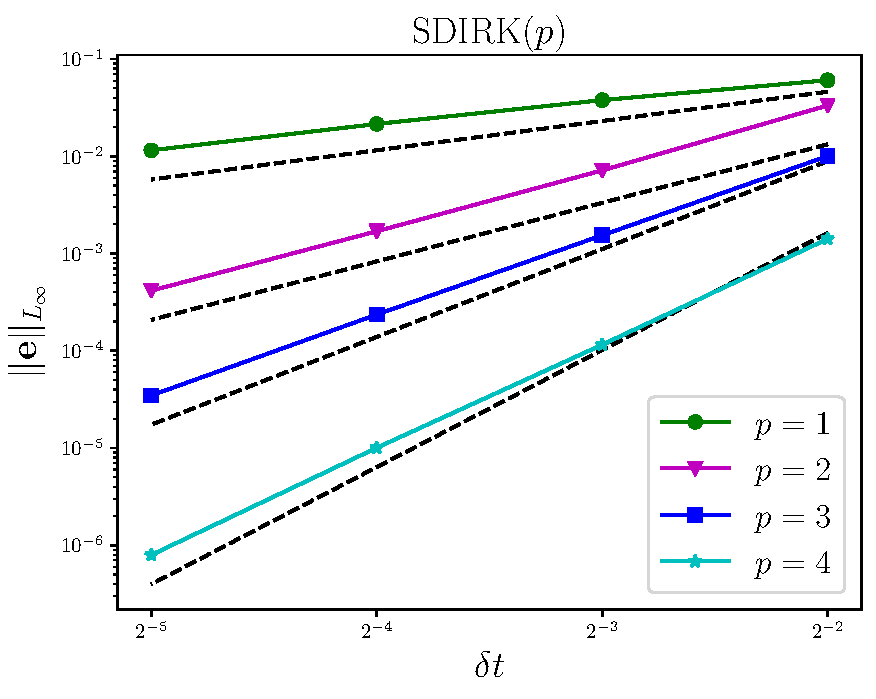
\includegraphics[width = 0.575\textwidth]{figures/SDIRK_d2_ex1}
\quad
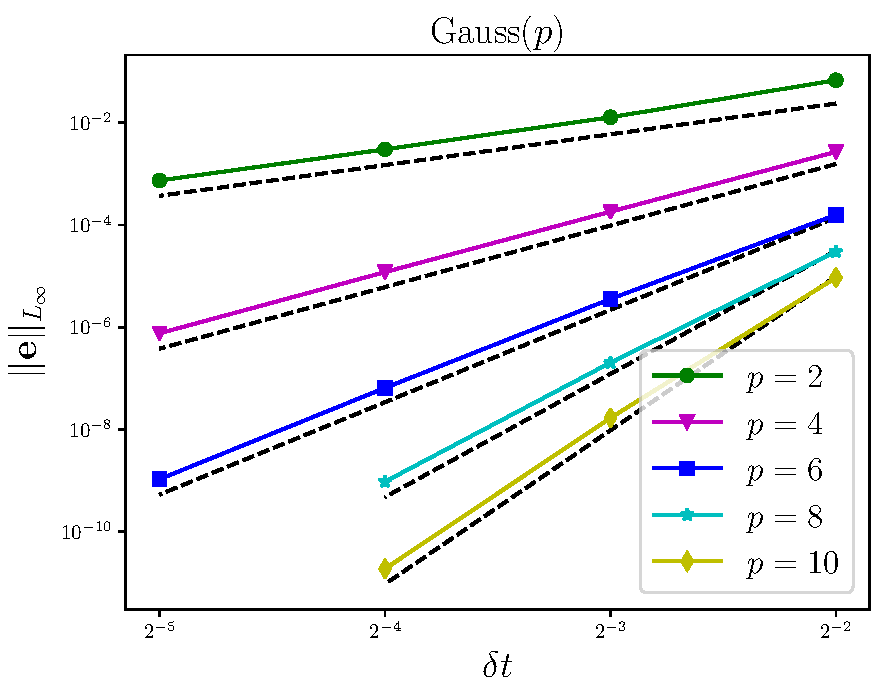
\includegraphics[width = 0.575\textwidth]{figures/Gauss_d2_ex1}
}
\centerline{
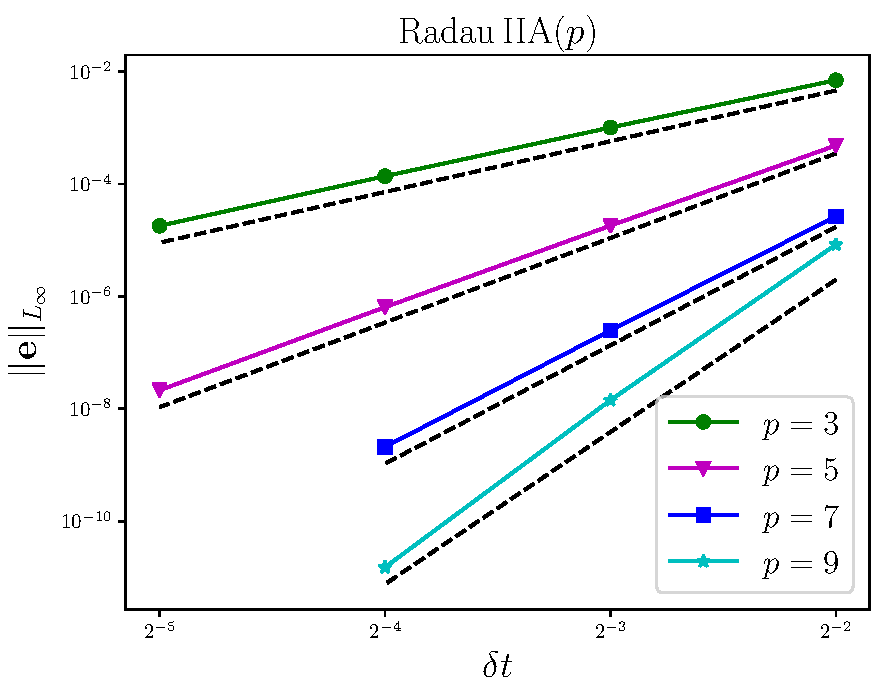
\includegraphics[width = 0.575\textwidth]{figures/RadauIIA_d2_ex1}
\quad
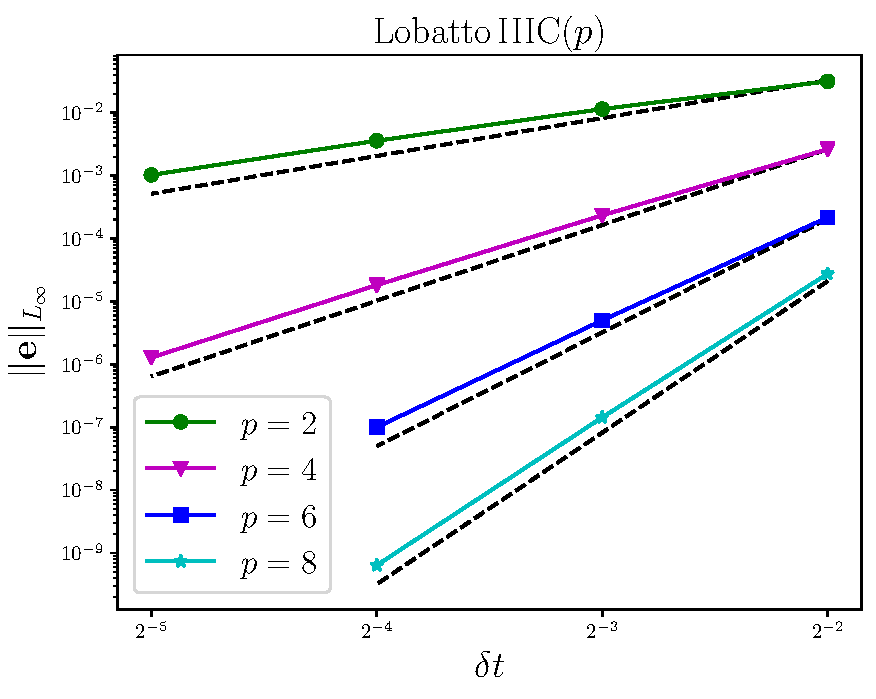
\includegraphics[width = 0.575\textwidth]{figures/LobattoIIIC_d2_ex1}
}
\caption{$L_{\infty}$ errors measured at $t \approx 2$. Theoretically predicted convergence rates of ${\cal O}(p)$ are shown as dashed black lines. ${\cal O}(p)$ IRK schemes are paired with ${\cal O}(p)$ spatial discretizations (or ${\cal O}(p+1)$ if $p$ is odd), and $\delta t = 2 \delta x$. 
\label{fig:errors2D}
}
\end{figure}


\begin{figure}[H]
\centerline{
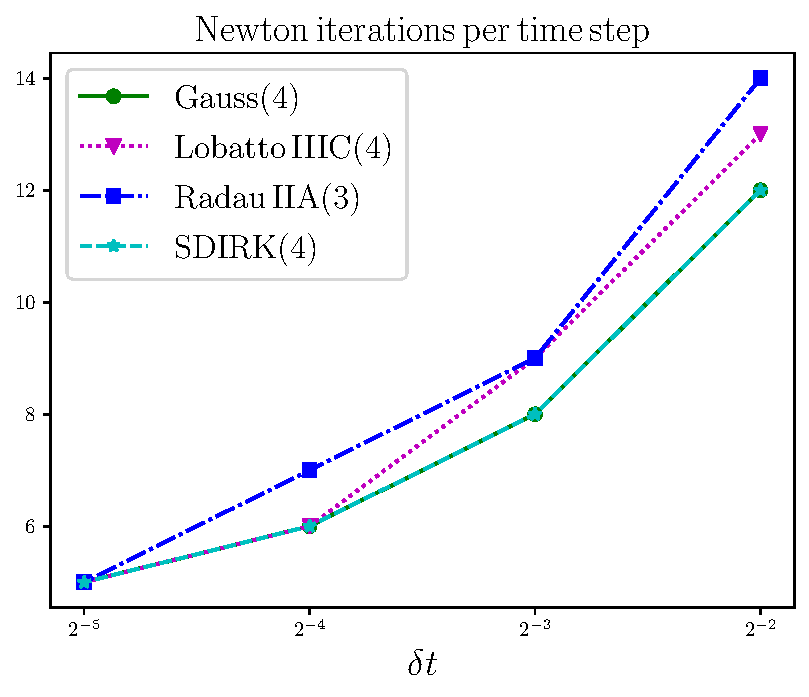
\includegraphics[width = 0.575\textwidth]{figures/newton_iters_O4}
\quad
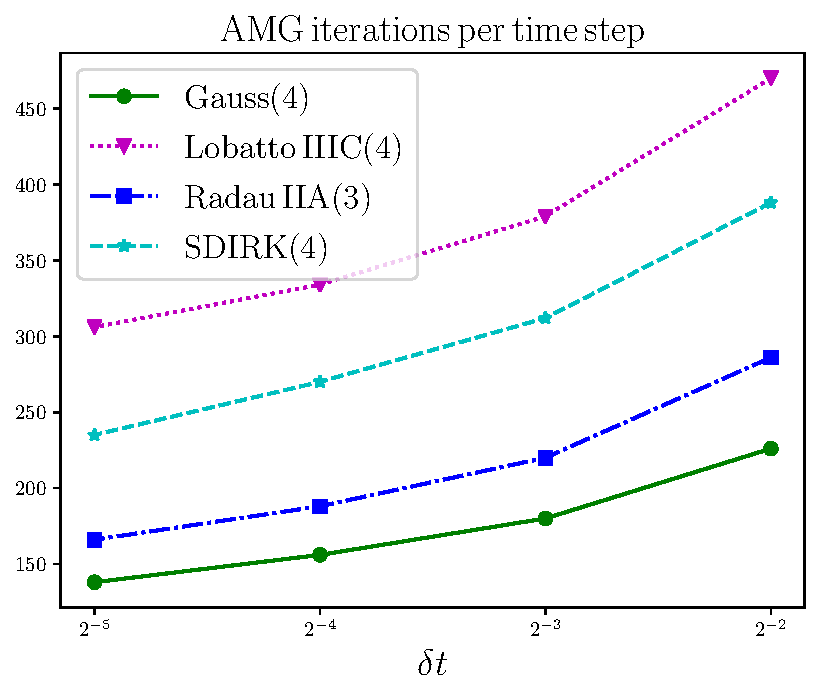
\includegraphics[width = 0.575\textwidth]{figures/amg_iters_O4}
}
\centerline{
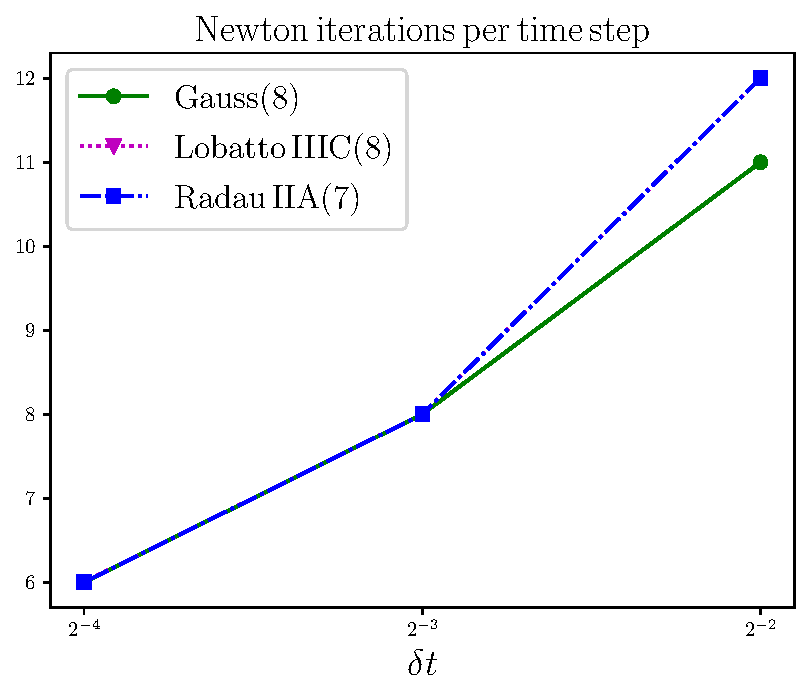
\includegraphics[width = 0.575\textwidth]{figures/newton_iters_O7}
\quad
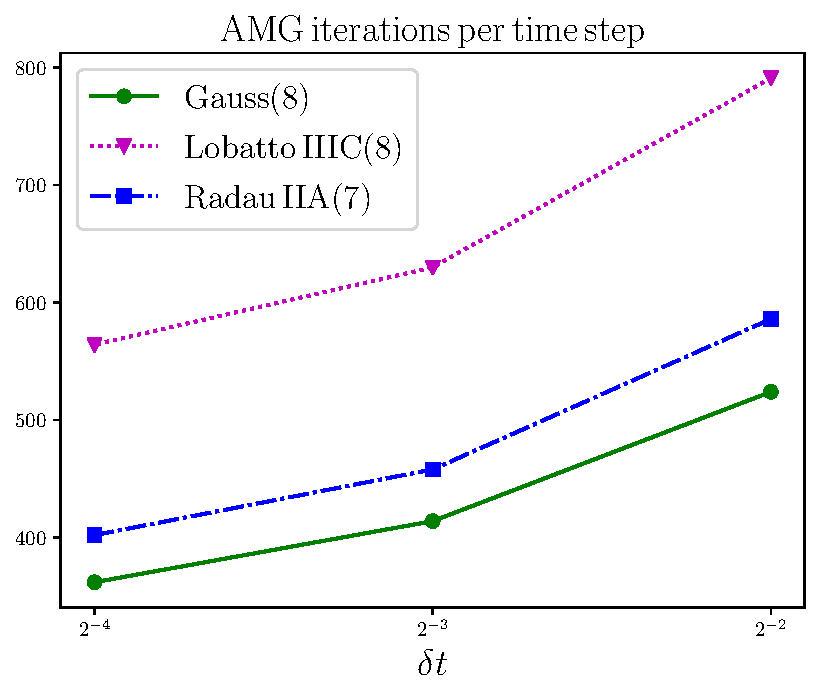
\includegraphics[width = 0.575\textwidth]{figures/amg_iters_O7}
}
\caption{Average iterations per time step (data associated with convergence plots in Figure \ref{fig:errors2D}). \textbf{Top:} 4th(ish)-order schemes. \textbf{Bottom:} 8th(ish)-order schemes. \textbf{Left:} Newton. \textbf{Right:} AMG. The systems that AMG is applied to have dimension $n = (16^2, 32^2, 64^2, 128^2)$ for $\delta t = (2^{-2}, 2^{-3}, 2^{-4}, 2^{-5})$. \tcp{Not really sure why so many Newton iterations decrease with resolution... See also Figure \ref{fig:iters1D}.}. In terms of work done per accuracy, it seems  Gauss $<$ Radau IIA $\ll$ Lobatto IIIC.
\label{fig:iters2D}
}
\end{figure}


\begin{figure}[H]
\centerline{
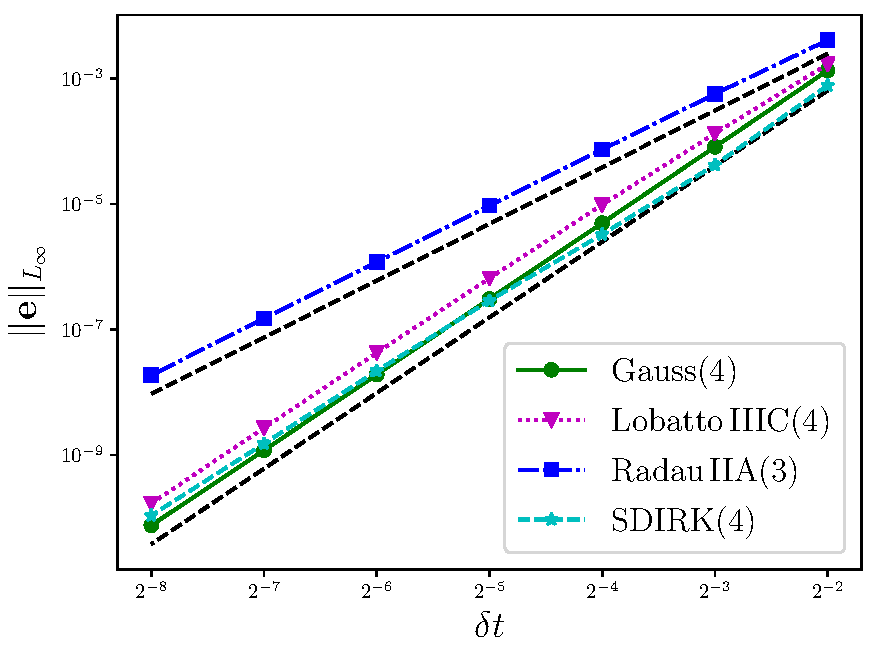
\includegraphics[width = 0.575\textwidth]{figures/errors_iters_O4_dim1}
}
\centerline{
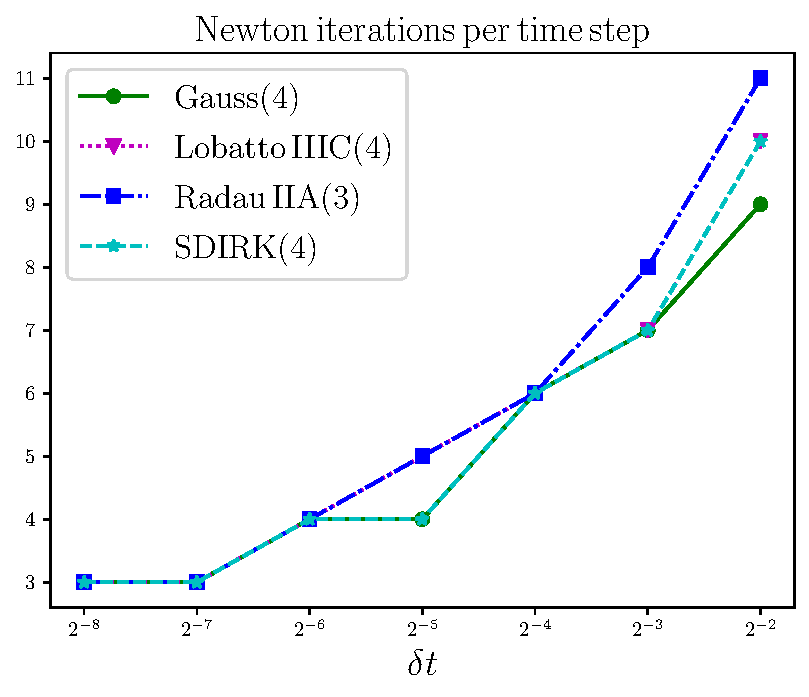
\includegraphics[width = 0.575\textwidth]{figures/newton_iters_O4_dim1}
\quad
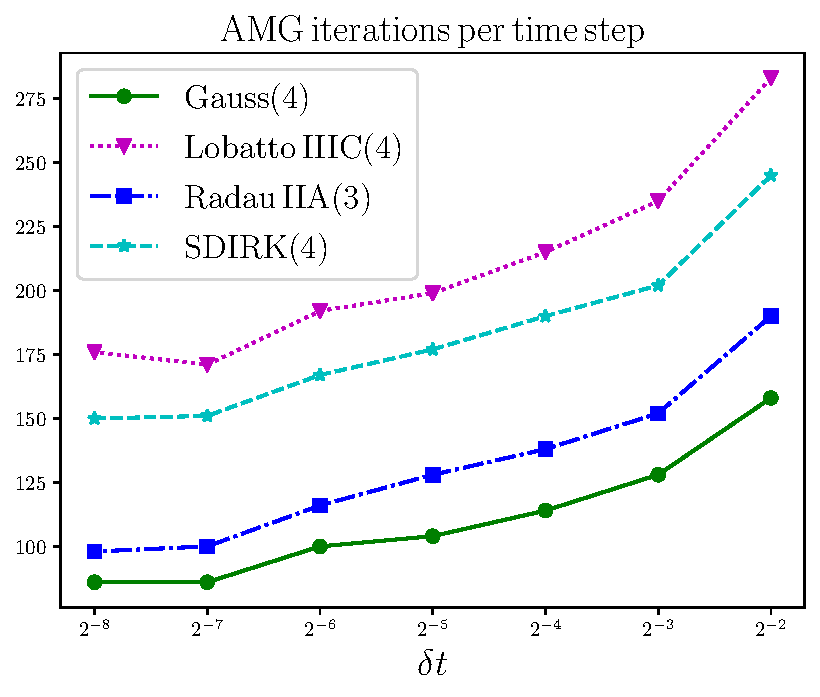
\includegraphics[width = 0.575\textwidth]{figures/amg_iters_O4_dim1}
}
\caption{Average iterations per time step for 4th(ish)-order discretizations of the \textbf{1D problem}, $u_t + 0.85 u^2_x = 0.3u_{xx} + s(x,t)$. 
\label{fig:iters1D}
}
\end{figure}


\end{document}


